\documentclass[aps,pra,showpacs,notitlepage,onecolumn,superscriptaddress,nofootinbib]{revtex4-1}
\usepackage[utf8]{inputenc}
\usepackage[tmargin=1in, bmargin=1.25in, lmargin=1.5in, rmargin=1.5in]{geometry}
\usepackage{amsmath, amssymb, amsthm}
\usepackage{graphicx}
\usepackage{xcolor}
\usepackage{enumitem}
\usepackage{datetime}
\usepackage{hyperref}
\usepackage{titlesec}
\usepackage{import}
\usepackage{mathtools}
\usepackage{thmtools,thm-restate}
\usepackage{comment}


% package for commutative diagrams
% \usepackage{tikz-cd}

%%%%%%%%%%%%%%%%%%%%%%%%%%%%%%%%%%%%%%%%%%%%%
\definecolor{crimson}{RGB}{186,0,44}
\definecolor{moss}{RGB}{0, 186, 111}
\newcommand{\pop}[1]{\textcolor{crimson}{#1}}
\newcommand{\zcom}[1]{\noindent\textcolor{crimson}{(Z): #1}}
\newcommand{\jcom}[1]{\noindent\textcolor{moss}{(J): #1}}
\newcommand{\wt}[1]{\widetilde{#1}}
\newcommand{\pqeq}{\succcurlyeq}
\newcommand{\pleq}{\preccurlyeq}
\newcommand{\hhrulefill}{\hspace{-1em} \hrulefill}

%%%%%%%%%%%%%%%%%%%%%%%%%%%%%%%%%%%%%%%%%%%%%
\hypersetup{
    colorlinks,
    linkcolor={crimson},
    citecolor={crimson},
    urlcolor={crimson}
}

\usepackage{qcircuit}

%%%%%%%%%%%%%%%%%%%%%%%%%%%%%%%%%%%%%%%%%%%%%
\theoremstyle{definition}
\newtheorem{definition}{Definition}[section]
\newtheorem{lemma}{Lemma}[section]
\newtheorem{theorem}{Theorem}[section]
\newtheorem{corollary}{Corollary}[theorem]
\newtheorem*{theorem*}{Theorem}
\newtheorem*{corollary*}{Corollary}
\newtheorem{remark}{Remark}[section]
\newtheorem{conjecture}{Conjecture}[section]
\newtheorem{example}{Example}[section]
\newtheorem{reminder}{Reminder}[section]
\newtheorem{problem}{Problem}[section]
\newtheorem{question}{Question}[section]
\newtheorem{answer}{Answer}[section]
\newtheorem{fact}{Fact}[section]
\newtheorem{claim}{Claim}[section]

\usepackage{geometry}
\geometry{
  left=25mm,
  right=25mm,
  top=20mm,
}
\usepackage{mathtools}

%%%%%%%%%%%%%%%%%%%%%%%%%%%%%%%%%%%%%%%%%%%%%
\bibliographystyle{unsrt}

%%%%%%%%%%%%%%%%%%%%%%%%%%%%%%%%%%%%%%%%%%%%%
%%%%%%%%%%%%%%%%%%%%%%%%%%%%%%%%%%%%%%%%%%%%%
%%%%%%%%%%%%%%%%%%%%%%%%%%%%%%%%%%%%%%%%%%%%%
\begin{document}

\title{Discrete Riemann surfaces and the Ising model: notes}
\author{Jack Ceroni}
\email{jackceroni@gmail.com}

\date{\today}

\maketitle

\section{Introduction}

\noindent The goal of these notes is to summarize and explain in greater detail the ideas outlined in Christian Mercat's paper \emph{Discrete Riemann surfaces and the Ising model}.

\section{Introducing the terminology of discrete surfaces}

\noindent We begin by letting $\Sigma$ be an oriented surface without boundary. In these notes, we will in addition assume that $\Sigma$ is a smooth manifold (it has a smooth structure which
has smooth transition maps). Let us begin by recalling a basic definition.

\begin{definition}[Equivalent definitions of an orientation]
  The most common definition for the orientation of a smooth manifold, and the one most likely known by the reader, is the following.
  Given a manifold $M$, an \emph{oriented atlas} of $M$ is an atlas of open neighbourhoods and associated coordinate charts, $(U_{\alpha}, \varphi_{\alpha})_{\alpha \in I}$
  such that each transition map $\varphi_{\alpha} \circ \varphi_{\beta}^{-1}$ (which is assumed to be $C^{\infty}$ as $M$ is smooth) has positive Jacobian determinant everywhere.
  An \emph{orientation} on a manifold is a smooth structure (a maximal smooth atlas) which is oriented.

  Equivalently, \pop{TODO: fill this in}
\end{definition}

\subsection{Introducing cell complexes}

\noindent We now come to the first set of definitions. In particular, we develop a means of placing a discrete, lattice-like structure on an otherwise continuous surface,
in such a way that the underlying geometry of the surface is repsected.

\begin{definition}[Cellular decomposition]
  Given $\Sigma$ as defined above (an oriented surface without boundary), a \emph{cellular decomposition} $\Gamma$ of $\Sigma$ is a partition of $\Sigma$ into disjoint connected
  sets (which we call cells) of three different types:
  \begin{itemize}
  \item A discrete set of points. We call these the \emph{vertices} of $\Gamma$, and denote them by $\Gamma_0$
  \item A collection of non-intersecting sets of the form $\gamma((0, 1))$, where $\gamma : [0, 1] \rightarrow \Sigma$ is a bijective path such that $\gamma(0)$ and $\gamma(1)$, the endpoints of the path, are contained
    in $\Gamma_0$. We will assume that any such $\gamma$ is also smooth, in the sense that each $\varphi_{\alpha} \circ \gamma$ is smooth for $x \in \gamma((0, 1)) \cap U_{\alpha}$, where $(U_{\alpha}, \varphi_{\alpha})$ is a coordinate chart
    of the smooth structure on $\Sigma$. We call these the \emph{edges} of $\Gamma$ and denote them by $\Gamma_1$.
  \item A collection of topological discs of the form $B$ (in other words, an embedding of an open ball $B^2$ in $\Sigma$)
    such that $\partial B$ can be written as a finite union of elements of $\Gamma_0$ and $\Gamma_1$ (nodes and edges). We call these the \emph{faces} of $\Gamma$, and denote them by $\Gamma_2$.
  \end{itemize}
  A cellular decomposition is said to be \emph{locally finite} if every compact subset $C$ of $\Sigma$ intersects only a finite number of elements of $\Gamma$.
\end{definition}

\begin{center}
  \begin{figure}
    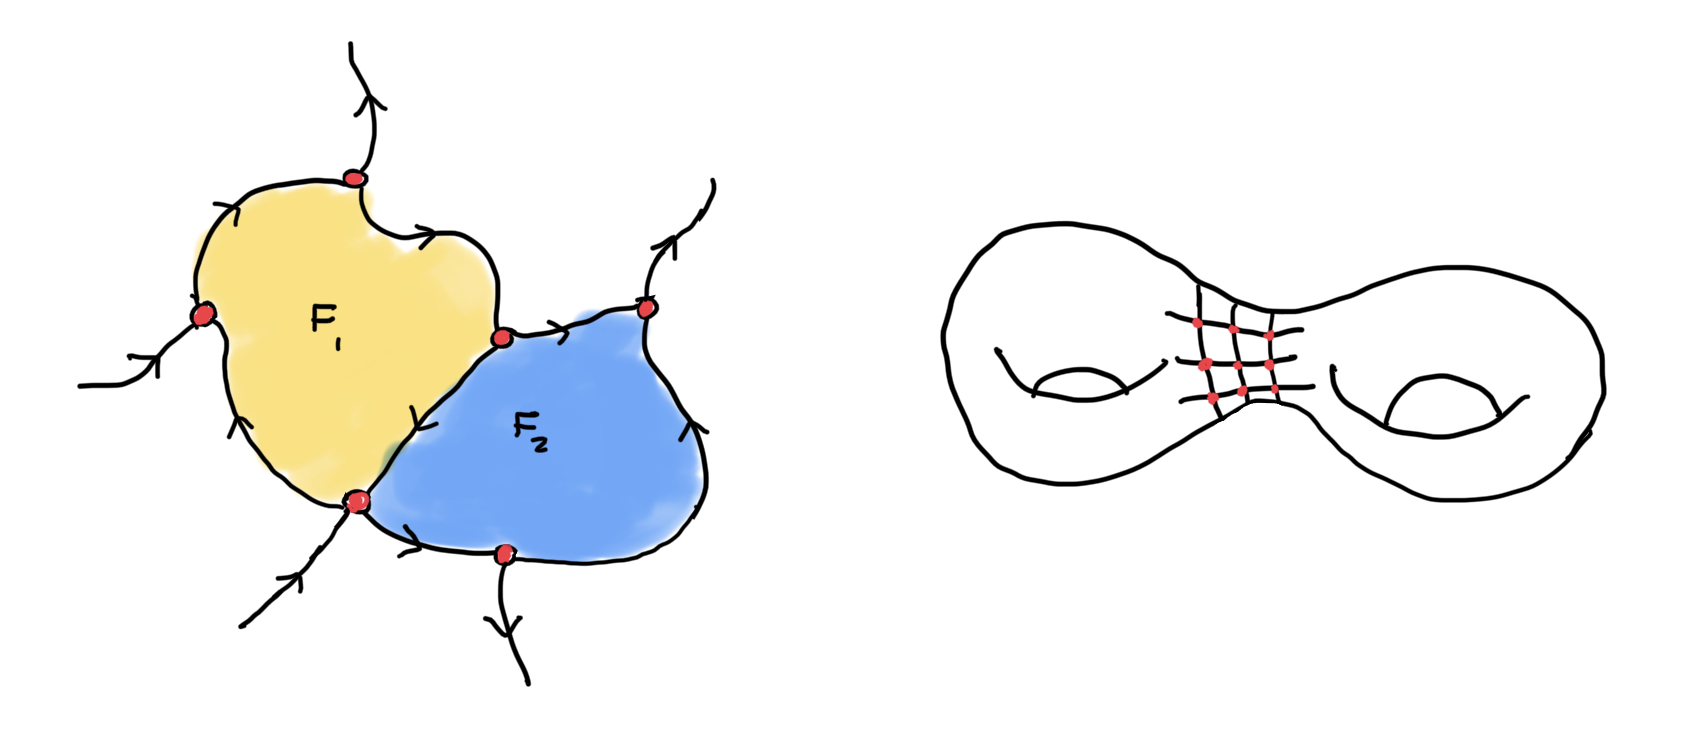
\includegraphics[width=400pt]{./assets/mercat1.jpeg}
    \caption{The left image depicts two faces $F_1$ and $F_2$ and their bounding, oriented edges (and vertices) of some cellular decomposition $\Gamma$. The right picture shows
    some of the cells of a cellular decomposition $\Gamma$ of a genus-$2$ surface $\Sigma$.}
    \end{figure}
  \end{center}

\begin{remark}[Parameterizing $\Gamma$]
  Note that the vertices, edges and faces of a cellular decomposition $\Gamma$ are all images of a $0$-ball (a point), $1$-ball (the interval $(0, 1)$), and $2$-ball (the set $\{x \in \mathbb{R}^2 \ | \ |x| < 1\}$), respectively,
  with respect to given parameterizations. This follows directly from the definition, with the edges being images of $(0, 1)$ and faces being embeddings of $B^2$. Equivalently, we can choose parameterizations which map from each element
  of $\Gamma$ to topological balls instead.
\end{remark}

\begin{remark}[Orientation of $\Gamma$]
Since each face in $\Gamma$ is an open subset of $\Sigma$, each will naturally inherit the orientation of the larger surface $\Sigma$. On the other hand, the edges of $\Gamma$
are not open in $\Sigma$: they, along with their vertex endpoints, make up the boundaries of the faces. Thus, the edges are not equiped with a canonical orientation, so
we instead arbitrarily choose one of the \emph{two possible} orientations (each edge is an orientable and path-connected manifold, so there are precisely two choices of orientation).
\end{remark}

\noindent We continue by translating a well-known construction from standard differential geometry to its discrete counterpart.

\begin{definition}
  We define the space of \emph{chains} on $\Gamma$, $C(\Gamma)$, as the $\mathbb{Z}$-module generated by taking formal linear combinations of cells of $\Gamma$.
  We define the space of $k$-chains on $\Gamma$, $C_k(\Gamma)$, to be the $\mathbb{Z}$-module generate by all dimension-$k$ cells (when each cell individually is treated as a manifold).
  This leads to a natural collection of boundary operators, $\partial : C_k(\Gamma) \rightarrow C_{k - 1}(\Gamma)$, so that we have the following complex
  \begin{equation}
    C_2(\Gamma) \xrightarrow{\qquad \partial \qquad} C_1(\Gamma) \xrightarrow{\qquad \partial \qquad} C_0(\Gamma).
  \end{equation}
  To be more specific, $\partial$ is a linear map which takes a formal linear combination of $k$-cells to a formal linear combination, with the same
  coefficients, of the corresponding boundaries
  \begin{equation}
    \partial (c_1 S_1 + \cdots + c_k S_k) = c_1 \partial S_k + \cdots + c_k \partial S_k
  \end{equation}
  where $S_j \in \Gamma$ for each $j$. Note that $\partial \circ \partial = 0$, as given a formal sum of faces, edges and vertices, the
  boundary will be a formal sum of edges and vertices.
\end{definition}



\section{Discrete holomorphic functions}

\section{A discrete deRham complex}

\section{A discrete Hodge star}

\section{Hodge's theorem for discrete surfaces}

\end{document}
